% A blossom and its contraction (generated by figs_c2ch06.py).
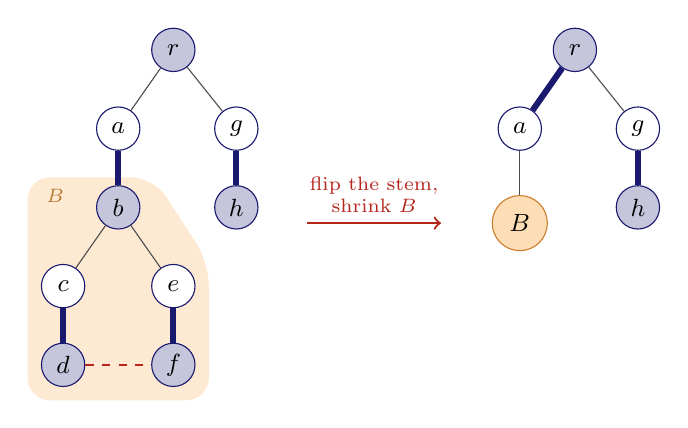
\begin{tikzpicture}[x=1cm,y=1cm,every node/.style={font=\small}]
\tikzset{ev/.style={circle,draw=MidnightBlue,fill=MidnightBlue!25,inner sep=1pt,minimum size=0.55cm},
  od/.style={circle,draw=MidnightBlue,fill=white,inner sep=1pt,minimum size=0.55cm},
  mt/.style={line width=2.2pt,MidnightBlue}, um/.style={thin,black!70}}
\fill[BurntOrange!15,rounded corners=8pt] (-0.65,-1.62) -- (0.95,-1.62) -- (1.65,-2.7) -- (1.65,-4.45) -- (-0.65,-4.45) -- cycle;
\node[ev] (r) at (1.2,0) {$r$};
\node[od] (a) at (0.5,-1.0) {$a$};
\node[ev] (b) at (0.5,-2.0) {$b$};
\node[od] (c) at (-0.2,-3.0) {$c$};
\node[ev] (d) at (-0.2,-4.0) {$d$};
\node[od] (e) at (1.2,-3.0) {$e$};
\node[ev] (f) at (1.2,-4.0) {$f$};
\node[od] (g) at (2.0,-1.0) {$g$};
\node[ev] (h) at (2.0,-2.0) {$h$};
\draw[mt] (a) -- (b);
\draw[mt] (c) -- (d);
\draw[mt] (e) -- (f);
\draw[mt] (g) -- (h);
\draw[um] (r) -- (a);
\draw[um] (b) -- (c);
\draw[um] (b) -- (e);
\draw[um] (r) -- (g);
\draw[BrickRed,thick,dashed] (d) -- (f);
\node[font=\scriptsize,BurntOrange!70!black] at (-0.3,-1.85) {$B$};
\draw[->,thick,BrickRed] (2.9,-2.2) -- node[above,font=\scriptsize,align=center] {flip the stem,\\ shrink $B$} (4.6,-2.2);
\node[ev] (r2) at (6.3,0) {$r$};
\node[od] (a2) at (5.6,-1.0) {$a$};
\node[ev,draw=BurntOrange!80!black,fill=BurntOrange!25,minimum size=0.7cm] (B2) at (5.6,-2.2) {$B$};
\node[od] (g2) at (7.1,-1.0) {$g$};
\node[ev] (h2) at (7.1,-2.0) {$h$};
\draw[mt] (r2) -- (a2);
\draw[um] (a2) -- (B2);
\draw[mt] (g2) -- (h2);
\draw[um] (r2) -- (g2);
\end{tikzpicture}
